
% PAGES: 5
\chapter{Introduction}
\label{mt:c:introduction}

%\begin{wrapfigure}{r}{5cm}
  %\centering
  %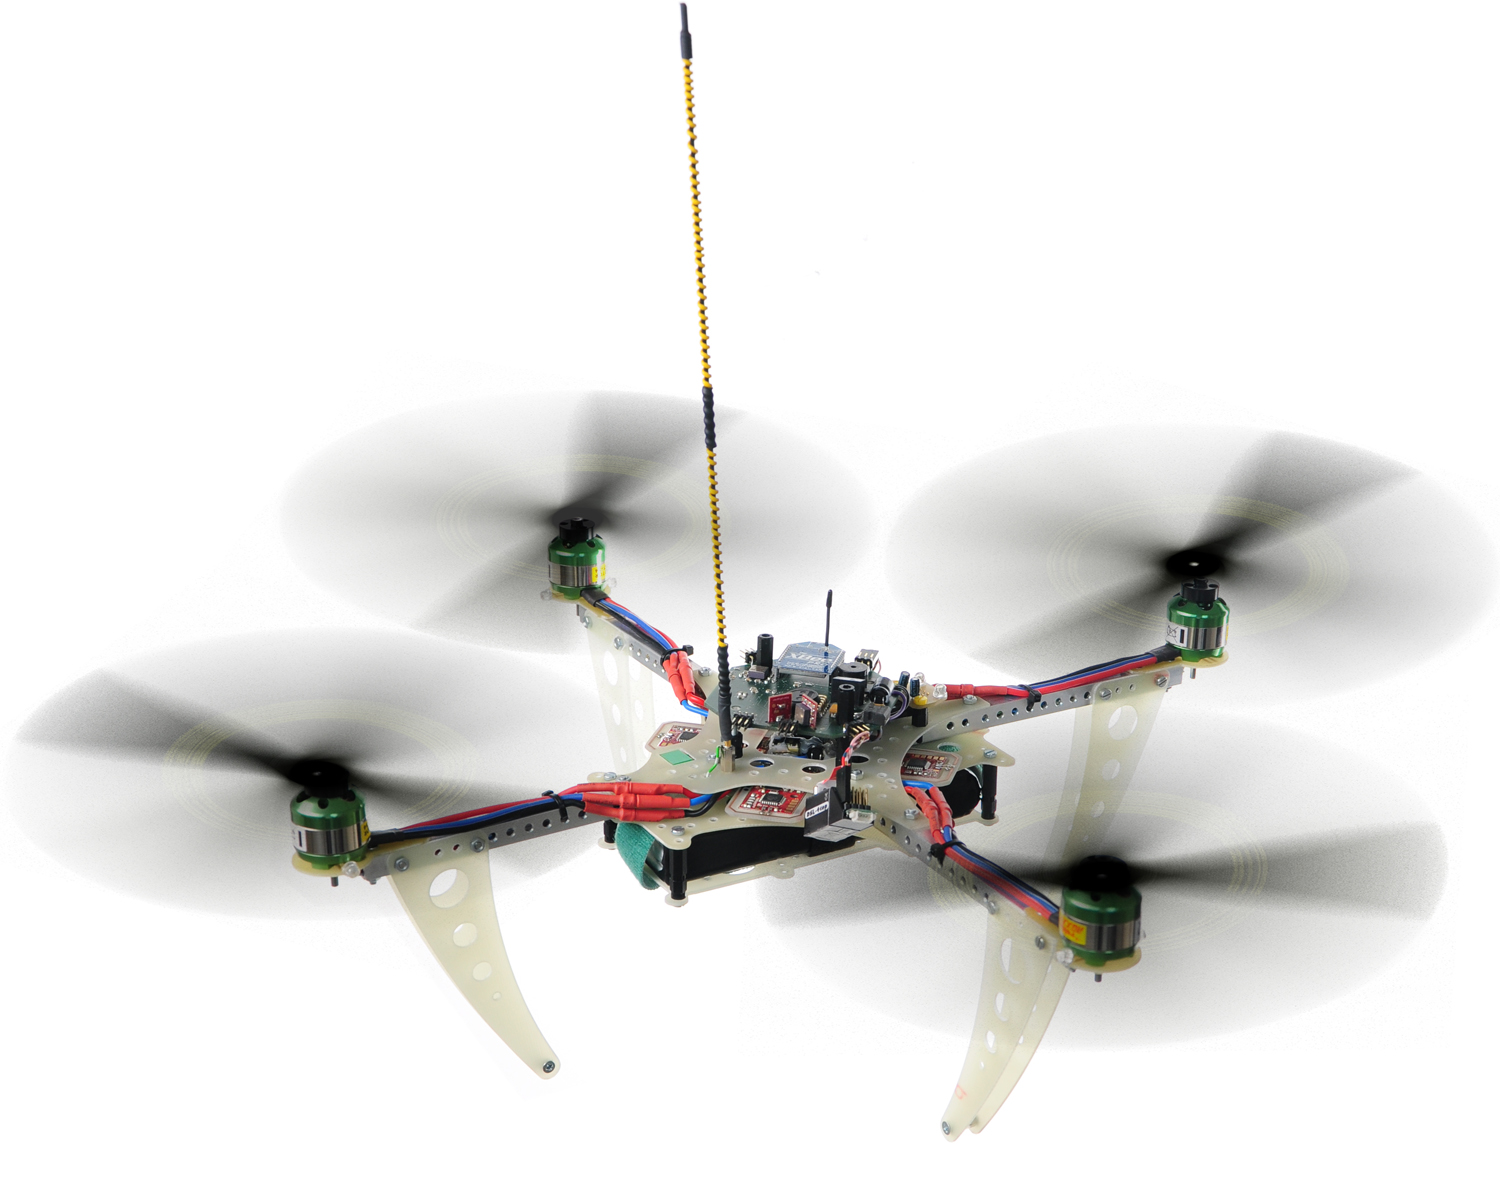
\includegraphics[width=0.5\textwidth]{graphic/QuadrocopterV3.jpg}
  %\caption {HSE Quadrocopter}
  %\label{fig:QuadrocopterV3.jpg}
%\end{wrapfigure}

In recent years, the interest in robotic science and the development of
robots enormously increased. Reasons for that are the unstoppable technological
progress in hard-and software techniques, but also the ambition to replace
humans with machines in dangerous, monotonous or unreachable industrial
environments (medical, space, aviation and so forth).
One area of these interests
is the aerial platform and the realization of \gls{UAV}, which are mostly controlled
via remote control or fly autonomous. These aircraft vehicles have several
capabilities, like in military or rescue operations, with special environments like
a burning house. For such indoor operation, it is important to
realise that some kinds of feedback sensors, like GPS-sensors, could not work
satisfactory. In such cases, \gls{UAV} face problems with their self-stabilization,
because their physical behaviour is generally unstable 
\citebib[p.1 Introduction]{BloWeiScaSie10}. Most of the attempts to stabilize
\gls{UAV} work with a clever combination of sensor equipment and control algorithms.
Mostly this controller uses an \gls{IMU} which is mounted on board and includes
acceleration sensors to detect movements in the given \gls{DOF}.
\newpage
Current acceleration
sensors, which are used for this purpose, are \gls{MEMS} or fiberoptic sensors which
have a finite precision and unacceptable error propagation in case of integration
for velocity or position detection 
\citebib[pp.11-13 Function Principles of MEMS, Sources of Error]{Fac08}.
 This problem also is a field of research for the Quadrocopter project of the
 \gls{HSE} \citebib[Website]{HSE10}. The goal of this Master's Thesis is to
research the topic of flight stabilisation and error drift elimination with an
optical sensor. This approach has to be tested and evaluated with the implementation of
a simulation focused on the behaviour of the flight dynamics in relation to the 
quality of the optical measurements and the control system of the quadrocopter.  

\begin{figure}[!h]
	\centering
		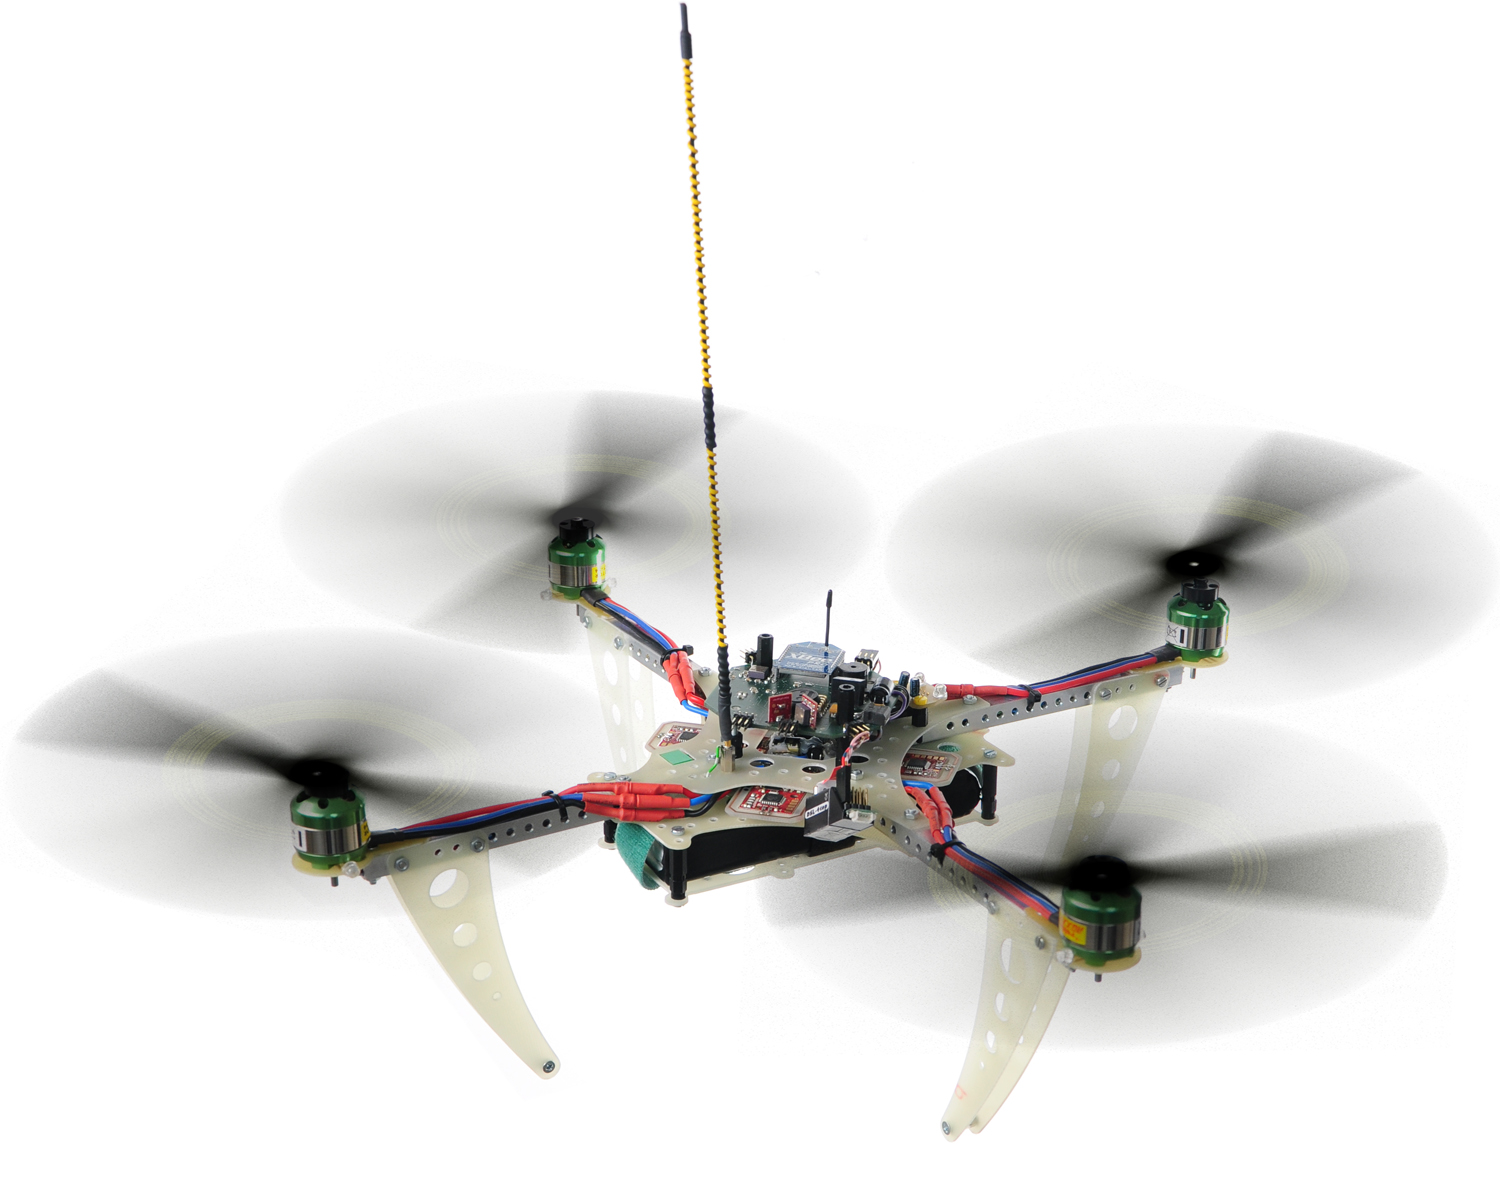
\includegraphics[width=0.8\textwidth]{graphic/QuadrocopterV3.jpg}
	\caption{HSE Quadrocopter}
	\label{fig:QuadrocopterV3.jpg}
\end{figure}

\newpage
\section{Context of the Project}

The quadrocopter project of the \gls{HSE} was launched with the goal to build a
system from the scratch, which is developed by students, scientific workers and
Professors. In a prior project, the \gls{PCB}, which contains
the parts necessary to control the quadrocopter, was designed by students at the
faculty of Mechatronics and Electrical Engineering in Goeppingen. Back then, these project
groups' focuses were on the simulation, implementation of basic functions
and visualization of the actual condition of the aircraft. The first two project
groups already show the their results, a multidisciplinary development
including hardware design, application development, embedded programming,
simulation and the interfaces between these special fields. In the year
2009, the Faculty of Information Technology adopted the development of the
project, with the aim to solve problems which came up in the previous development process
and to redesign the soft- and hardware architecture. So a new hardware design was
developed in a corporation between the two faculties, with the outcome of a \gls{CCU}
which can detect inertial movements in six \gls{DOF} and can control the four
actuators of the quadrocopter via so-called "brushless controllers".
One of the biggest unresolved problems so far is the development of a robust
controller and the elimination of drifts, which especially come up at the hovering state.
 The practice and experience of previous developments show that it is
indispensable to proof new developments with a simulation before they will be
realized at the real \gls{UAV}. So the main topic and focus of this Master's
Thesis will be on the development of a simulation that shows potential solutions
of the mentioned problems, and the research and evaluation for the outcome results.

\section{Problem Description}

Improvements in high density power storage, integrated miniature actuators and
sensors facilitate the development of \gls{MAV} and new areas of research for
unmanned and autonomous flying systems \citebib[p.1 Introduction]{BourMurSie04}.
 This new area of interest also brought a new area of problems.
 One of these is the fact that the pilot of the aerial vehicle does not exist, either
 because the \gls{UAV} flies autonomous or because the pilot observes and controls the \gls{UAV} via
 remote control. In both cases, it is necessary that the \gls{UAV} system can detect
 its absolute position, to provide the pilot with a better quality of control or,
 furthermore, to manoeuvre autonomous. The following articles also describe this
 problem with different views and approaches 
\citebib[p.2 Localization and path planning]{GrzGriBur09}
\citebib[p.1 High precision aircraft positioning]{WenMasZel10} 
\citebib[p.2 Teleoperated Robot Control]{BluHolLinMolSurViaTre08}.

This necessity of location determination leads to the requirement of a measurement unit which
provides the possibility to detect the movements in the given \gls{DOF}. Because of low-cost
and low-complexity reasons, the most popular components which are used to reach
a nearly satisfactorily level of flight stabilisation are inertial sensors.
These sensors, altogether called \gls{IMU}, have the ability to detect the
acceleration or velocity of translational or rotational movements. Furthermore, a control
system can be used in a closed loop together with the \gls{IMU} and theoretically can
 correct nearly every disturbance in a continual system 
\citebib[pp.45-64 System Control]{Bou07}
\citebib[pp.49-51 Control Strategy]{CasLozAle05}.
\newpage
The resolution limitation of the sensors and the necessity of integrating the
acceleration values for position and velocity determination have
a big impact in aspects of error propagation and detection of smoothly movements
in real systems \citebib[p.5 Low-acceleration Drift]{Tip08}.
The quadrocopter of the \gls{HSE} also includes an \gls{IMU} for stabilisation and faces 
the same problems. These problems can be eliminated with the extension of an optical system,
which can track the absolute position of the \gls{UAV} ego-motion. 

%\section{Approach}
%Evaluation and critically assessment of approaches.
%Simualtion of existing hardware
%Simulation of a distributed Ego motion camera system 
%Simulation of needed control system

\section{Aims and Objectives}

The aim of this dissertation is to provide a simulation architecture that can be
used as prototype development platform for a distributed visual movement
detection and control of a quadrocopter. Furthermore, the characteristics of the
distributed image processing and movement detection have to be analysed in
relation to the variation of configurations and critically assessed.

One essential objective is for the configuration of the simulating components
to provide the option to simulate a range of hardware components that have not been
purchased yet. By way of example, the simulation of the on-Board camera has
to provide options of configuration for the image size, underground structure and
so on. The simulation of the communication between \gls{UAV} and host also has to
provide a variation of transmission rate, or abstracted as frame rate, and further behaviour which could affect
the visual movement detection at the base station. The efficiency in relation
with the quality of functionality is an important indicator for the success and acceptance of
the distributed movement detection approach. 
\newpage
Therefore it is important to get an insight
on the possible characteristics of the simulated components with the result to
find a solution that satisfies the efficiency and quality aspects.

Another important objective is for the interfaces between the simulating
components to be clearly specified and allow a way of modular exchangeability of
simulation components with the real objects.
This purpose has to allow a more precise investigation of the behaviour of the real hardware related components, and the option to test software for the \gls{UAV} target, like the On-Board control
algorithm, at the base station.

The realisation of the simulation therefore has to provide an encapsulated and
flexible architecture, and has to simulate behaviour like delays and jitters for
simulated components. Thereby, the simulation has to adjust a real-time-behaviour
into the complete simulated environment and, allow measurements and predictions 
about feasibilities with the simulated configuration.
